%======================================================================
%  BACHELOR THESIS PROPOSAL
%  Ruhr-Universität Bochum — IT-Sicherheit / Informationstechnik
%
%  COMPILE:  pdflatex -> biber -> pdflatex -> pdflatex
%            (TeXstudio: F5 / "Build & View" with the default
%             pdflatex + biber tool chain)
%
%  Fill in the \newcommand values below, then write in sections/.
%======================================================================
\documentclass[11pt,a4paper]{article}

%----------------------------------------------------------------------
%  Metadata — EDIT THESE
%----------------------------------------------------------------------
\newcommand{\thesistitle}{Understanding Privacy Harm Communication in Fitness and Health Tracking Apps}
\newcommand{\thesissubtitle}{Thesis Proposal}
\newcommand{\authorname}{Hamza}
\newcommand{\matriculation}{TODO: matriculation number}
\newcommand{\supervisorone}{TODO: Prüfer*in (RUB)}
\newcommand{\supervisortwo}{Kavous Salehzadeh Niksirat, MPI-SP}
\newcommand{\thefaculty}{Faculty of Computer Science}
\newcommand{\theuniversity}{Ruhr-Universität Bochum}
\newcommand{\theprogram}{B.Sc. IT-Sicherheit / Informationstechnik}
\newcommand{\thesemester}{Winter Semester 2026/27}

%----------------------------------------------------------------------
%  Packages
%----------------------------------------------------------------------
\usepackage[utf8]{inputenc}
\usepackage[T1]{fontenc}
\usepackage[english]{babel}
\usepackage{lmodern}
\usepackage{microtype}

\usepackage[a4paper,margin=2.6cm]{geometry}
\usepackage{setspace}
\onehalfspacing

\usepackage{graphicx}
\graphicspath{{figures/}}
\usepackage{booktabs}
\usepackage{tabularx}
\usepackage{enumitem}
\usepackage{csquotes}

% The methodology overview figure is drawn in TikZ rather than included as an
% image, so there is no binary asset to keep in sync with the text.
\usepackage{tikz}
\usetikzlibrary{arrows.meta,positioning}

\usepackage{xcolor}
\definecolor{linkblue}{HTML}{16537E}
\usepackage[hidelinks]{hyperref}
\hypersetup{
  colorlinks = true,
  linkcolor  = linkblue,
  citecolor  = linkblue,
  urlcolor   = linkblue,
  pdftitle   = {\thesistitle},
  pdfauthor  = {\authorname}
}

%----------------------------------------------------------------------
%  Bibliography
%  Switch style to  style=apa  or  style=alphabetic  if your supervisor
%  prefers it (apa additionally needs the biblatex-apa package).
%----------------------------------------------------------------------
\usepackage[backend=biber,style=numeric-comp,sorting=nyt,maxbibnames=99,urldate=long]{biblatex}
\addbibresource{../_shared/references.bib}

%----------------------------------------------------------------------
%  Helper for TODOs — remove \todo lines before submitting
%----------------------------------------------------------------------
\newcommand{\todo}[1]{\textcolor{red}{\textbf{[TODO: #1]}}}

%----------------------------------------------------------------------
%  Repository paths. \nolinkurl lets long paths break across lines and
%  needs no escaping of _ inside the argument.
%----------------------------------------------------------------------
\newcommand{\pathname}[1]{\nolinkurl{#1}}

%======================================================================
\begin{document}

%---------------------------- Title page ------------------------------
\begin{titlepage}
\centering
\vspace*{2cm}

{\Large \theuniversity\par}
{\large \thefaculty\par}
\vspace{2.5cm}

{\Huge\bfseries \thesissubtitle\par}
\vspace{1cm}
{\LARGE \thesistitle\par}

\vspace{3cm}
\begin{tabular}{@{}ll@{}}
Author            & \authorname \\
Matriculation no. & \matriculation \\
Programme         & \theprogram \\[1em]
Supervisor        & \supervisorone \\
Co-supervisor     & \supervisortwo \\[1em]
Semester          & \thesemester \\
Date              & \today \\
\end{tabular}

\vfill
\end{titlepage}

%---------------------------- Abstract --------------------------------
\begin{abstract}
\noindent
% Abstract — write LAST. 150–200 words.
% One sentence each: context, gap, what you do, what you expect to find.
\todo{Write the abstract last.}

\end{abstract}

\newpage
\tableofcontents
\newpage

%---------------------------- Body ------------------------------------
%  The four sections the supervisor asked for come first, in order:
%  background -> research problem -> why it matters -> methodology.
\section{Background}
\label{sec:background}

\subsection{Self-tracking has become an ordinary data practice}

Health and fitness tracking is no longer a niche activity. In Germany,
73\,\% of smartphone users report using health apps to support fitness,
nutrition, or general wellbeing~\parencite{bitkom2025health}. The category is
broad: step and activity counters, sleep and heart-rate monitors, workout and
nutrition apps, and menstrual and fertility trackers. A wearable device may or
may not be involved. What is always involved is an app --- it is where data is
entered, displayed, stored, and transmitted. This is why the unit of analysis
in this thesis is the app and the communication surrounding it rather than the
hardware.

Three kinds of data accumulate. Users supply attributes directly: age, weight,
goals, symptoms, mood, sexual activity. Sensors produce continuous streams:
steps, heart rate, sleep phases, GPS traces. The system adds its own context:
timestamps, device identifiers, usage patterns~\parencite{gabriele2020understanding}.
What distinguishes tracking data from most other consumer data is that it is
longitudinal and involuntary in character --- once the app is installed, the
record keeps growing whether or not the user is thinking about privacy. Under
Article~9(1) of the General Data Protection Regulation, data concerning health
is a special category of personal data; menstrual and fertility data falls
squarely within it~\parencite{gdpr2016}.

\subsection{From data practices to privacy harms}

A \emph{privacy violation} and a \emph{privacy harm} are not the same thing.
Solove's taxonomy classifies the harmful \emph{activities} --- information
collection, processing, dissemination, and
invasion~\parencite{solove2006taxonomy}. Citron and Solove later classify the
\emph{injuries} those activities produce, and it is this second typology that
the present work builds on: physical, economic, reputational, psychological,
autonomy, discrimination, and relationship
harms~\parencite[830--861]{citron2021harms}. Calo had earlier drawn a related
line between the \emph{subjective} harm of perceived unwanted observation and
the \emph{objective} harm of information being used against a
person~\parencite{calo2011boundaries}.

What these typologies do not supply is the route from a system property to an
injury. Knabenhans et al.\ close that gap with \emph{harm
trees}~\parencite{knabenhans2026harms}. A tree links system components ---
information the functionality necessarily leaks, requirements the system
imposes on users --- to adversarial capabilities, and those capabilities to
harms. Their analysis of the European Digital Identity Framework isolates three
capabilities that follow from the core functionality itself: distinguishing
between users, tracking users, and inferring attributes about them. Crucially,
they separate pathways that are inherent to the functionality, pathways that
arise from deploying it in a digital context, and pathways that come from
concrete implementation choices --- and show that privacy-enhancing
technologies (PETs) can only close the last of the three. The same three
capabilities describe a health tracker well, which makes the model transferable
to this domain even though the original object of study is different.

That inference capability is not hypothetical here. Salehzadeh Niksirat et al.\
reviewed 236 studies of wearable activity trackers and report that tracker data
can be mined to infer private attributes, personality traits among
them~\parencite{niksirat2024wearable}.

\subsection{Modern risk is inference-centric, and so is PET marketing}

Martin, Nissenbaum, and Shmatikov examine three principles that underlie the
privacy techniques large technology companies have recently deployed:
limiting third-party access to personal data, minimising the use and retention
of raw data in favour of inferences drawn from it, and keeping personal data on
the user's device~\parencite{martin2025cookies}. Their objection is not that the
techniques fail on their own terms. It is that a technique can satisfy all
three principles while the privacy-violating behaviour continues untouched,
because the sensitive object is the inference, not the raw record. Their
vignette studies show that users' expectations do not follow the first
party\,/\,third party or raw data\,/\,inference distinctions that the principles
are built on.

For a health tracker this is the central point. Cycle length and symptom entries
support pregnancy inference; location and activity traces support inferences
about routine, workplace, and health status. Prior work on period trackers has
documented both the technical basis for such inferences and the concrete fears
users attach to them~\parencite{cao2024deleted,shipp2020period}.

\subsection{Where privacy is communicated}

Providers communicate privacy on several surfaces at once, and the surfaces
differ in audience, length, and legal weight:

\begin{enumerate}[leftmargin=*,itemsep=2pt]
  \item the \textbf{privacy policy}, the only surface with a direct legal
        mandate;
  \item the \textbf{store listing} --- the description text plus the structured
        disclosure that each platform requires (Google Play's Data Safety
        section, Apple's Privacy Nutrition Labels);
  \item the \textbf{provider's website and marketing material}, including
        advertisements and company privacy blog posts;
  \item the \textbf{app interface itself} --- onboarding screens, consent and
        permission dialogues, privacy settings, and the paths that lead to
        export or deletion.
\end{enumerate}

Each surface has known weaknesses. Policies are long enough that reading them is
economically irrational~\parencite{mcdonald2008cost}. Structured store
disclosures are self-reported and frequently wrong: a dynamic study of almost
5{,}000 Android apps found that 81\,\% misrepresented their data collection or
sharing practices in the Data Safety
section~\parencite{arkalakis2024abandon}, and a large-scale longitudinal study of
Apple's labels documents how unevenly they are created and
maintained~\parencite{li2022ios}.

\subsection{What the law asks providers to say}
\label{sec:law}

The transparency regime is built around describing \emph{what will be done with
data}. Articles 13 and 14 GDPR enumerate the controller's identity, the purposes
and legal basis of processing, recipients, third-country transfers, retention
periods, and data-subject rights~\parencite{gdpr2016}. Consequences appear in
exactly one narrow place: for automated decision-making within the meaning of
Article 22(1) and (4), Article 13(2)(f) requires \enquote{meaningful information
about the logic involved, as well as the significance and the envisaged
consequences of such processing for the data subject}. Breaches are addressed
reactively --- Article 34 obliges the controller to communicate a breach to
affected individuals, but only once it has occurred and only where it is likely
to result in a high risk to their rights and freedoms.

Nothing in the regime requires a provider to state what can be \emph{derived}
from the data it collects, or what would \emph{follow for the user} if that data
were exposed. This is the structural reason to expect silence on inference,
breach consequences, and incident handling --- and the reason that silence is
worth measuring rather than assuming.

\subsection{What prior work establishes, and where it stops}

Three strands of work bear on the question, and each stops short of it.

\paragraph{Stated practice versus actual practice.}
A substantial measurement literature compares what apps say with what they do.
Huckvale et al.\ found that 29 of 36 depression and smoking-cessation apps
transmitted data to services run by Google or Facebook while only 12 disclosed
this in a policy~\parencite{huckvale2019assessment}. Shipp and Blasco
systematically analysed the privacy policies of 30 Android menstrual
apps~\parencite{shipp2020period}. Malki et al.\ combined a thematic analysis of
Data Safety sections and privacy policies with a privacy-focused usability
inspection across 20 popular female mHealth apps and found inconsistencies
between policy text and in-app features, flawed consent and deletion mechanisms,
and covert collection of sensitive data~\parencite{malki2024exploring}. Hudig and
Singh analysed the network transmissions of eight fertility tracker products and
found data flowing to endpoints associated with organisations across several
countries~\parencite{hudig2025intimate}. At scale, MAPS audited
compliance across roughly a million apps~\parencite{zimmeck2019maps}. All of
these ask whether the disclosure is \emph{true}. None asks which \emph{harms} it
names.

\paragraph{What users know and expect.}
Gabriele and Chiasson surveyed 212 fitness tracker users: participants were
reasonably confident about \emph{what} data was collected but unsure \emph{how}
it was used, and when presented with scenarios carrying security and privacy
implications they judged them plausible yet
unlikely~\parencite{gabriele2020understanding}. Cao et al.\ surveyed 183 US
women after the overturn of Roe v.\ Wade and found high concern about period
tracker data practices combined with a feeling of being uninformed and powerless
about mitigation~\parencite{cao2024deleted}. These studies measure the belief;
they do not analyse the material that shapes it.

\paragraph{Methods for reading this material.}
Privacy policies have been a corpus-analysis object for a decade. The OPP-115
corpus established an annotation scheme for data practices in
policies~\parencite{wilson2016creation}; Polisis showed that those categories can
be predicted automatically~\parencite{harkous2018polisis}; and large language
models have since been evaluated for policy analysis at
scale~\parencite{rodriguez2024llm}. On the interface side, the cognitive
walkthrough offers a structured, task-based inspection
procedure~\parencite{wharton1994cognitive}, complementing heuristic
evaluation~\parencite{nielsen1994heuristic}. The annotation schemes these methods
carry, however, are schemes of \emph{data practices} --- collection, sharing,
retention, choice. None of them has a category for harm.

\section{Research Problem}
% State the gap in one paragraph, then make it precise.
%   Observation: privacy communication covers downstream data practices but is
%   largely silent on inference, breaches and incident handling.

\todo{State the gap.}

\subsection{Research Questions}
\begin{description}[leftmargin=2.2cm, style=nextline]
  \item[\textbf{RQ1}] \todo{...}
  \item[\textbf{RQ2}] \todo{...}
  \item[\textbf{RQ3}] \todo{...}
\end{description}

\subsection{Scope and Delimitations}
\todo{What is in scope (which app categories, which market, which sources) and
what is explicitly out of scope.}

\section{Significance of the Problem}
\label{sec:significance}

\subsection{For users: a vocabulary they are never given}

To decide whether to install a cycle tracker, a person has to weigh a benefit
they can feel against a risk they have to imagine. Privacy communication is the
main material they have for the second half of that judgement, and it is
material about mechanisms: categories of data, categories of recipient,
retention periods. If it never names a consequence, the user must supply the
consequence themselves.

The evidence suggests they cannot. Fitness tracker users are confident about
what is collected and unsure how it is used, and they rate harmful scenarios as
plausible but unlikely~\parencite{gabriele2020understanding}. Period tracker
users report high concern coupled with a sense of being uninformed and powerless
about what to do~\parencite{cao2024deleted}. That pattern --- concern without
actionable understanding --- is what one would predict from communication that
is complete about data flows and silent about stakes. Establishing whether the
silence is real, and where exactly it falls, turns a plausible explanation into
a measured one.

The risk is sharpest where inference is sharpest. A user who reads that an app
does not share raw data may reasonably conclude they are protected. If the
provider derives and acts on an inference instead, the conclusion is wrong, and
nothing in the text told them so~\parencite{martin2025cookies}.

\subsection{For providers and designers: a map of where communication fails}

Providers are not, in the main, choosing between honesty and deception; the
measurement literature already covers deception. They are choosing what to put
in a finite amount of text and screen space, and the conventions they inherit ---
from legal templates, from store label schemas --- have no slot for harm. A
systematic map of which harms are named, on which surface, and in what terms
gives design and policy teams something they currently lack: an account of what
their communication omits, expressed in categories a non-lawyer can act on.

There is already evidence that the design space exists. Hudig and Singh
co-designed ten concrete transparency and control mechanisms with fertility
tracker users~\parencite{hudig2025intimate}, and Malki et al.\ derive concrete
recommendations from the inconsistencies they
found~\parencite{malki2024exploring}. Both stop short of asking what the
communication should \emph{say about harm}; this thesis supplies that input.

\subsection{For regulators: evidence about a gap the law leaves open}

Section~\ref{sec:law} set out the structural point: the GDPR's
transparency articles enumerate practices, and require a statement of
consequences only in the narrow automated-decision-making case of Article
13(2)(f); breach communication under Article 34 is
reactive~\parencite{gdpr2016}. Platform disclosure schemas inherit the same
frame, and are in any case unreliable~\parencite{arkalakis2024abandon,li2022ios}.

Whether harm-facing disclosure would add anything is currently an untested
assumption in that debate. If providers turn out to name harms voluntarily and
in useful terms, the case for mandating it weakens. If, as expected, the four
elements identified in Section~\ref{sec:problem} are near-absent across an
entire market segment handling Article~9 special-category data, that is a
concrete, citable finding about the limits of a transparency regime built on
data-practice disclosure.

The structured platform disclosures do not fill the gap either. Both are
developer self-declarations against a fixed schema of data categories, which is
why their measured error rates are as high as they
are~\parencite{arkalakis2024abandon,li2022ios} --- and, more to the point here,
why no schema of that shape can carry a statement about harm in the first place.
What providers say in the free text, where nothing constrains them, is therefore
the half of the picture that no existing measurement covers.

\subsection{For research: extending harm analysis to provider discourse}

The harm literature has been developed in two places: in legal scholarship,
where the object is what a court will
recognise~\parencite{citron2021harms,calo2011boundaries,solove2006taxonomy}, and
in systems analysis, where the object is what a system's functionality makes
possible~\parencite{knabenhans2026harms}. Neither has been turned on the text
that providers actually put in front of users.

Doing so makes three contributions to method as well as to findings. It tests
whether a typology built for adjudication can be operationalised as a coding
scheme for corporate prose --- a question with an answer either way. It extends
usable-privacy document analysis, whose annotation schemes are schemes of data
practices~\parencite{wilson2016creation,harkous2018polisis}, with a harm
dimension. And it joins document analysis to interface inspection in one design,
so that what a provider writes can be compared with what the same provider
shows~\parencite{wharton1994cognitive}, which is where RQ4 lives.

\section{Methodology}
\label{sec:method}

\subsection{Overview}

The study is a structured content analysis of privacy communication, combined
with a task-based inspection of the interfaces that carry part of that
communication. It proceeds in four steps: build a frozen sample of apps; collect
every privacy-relevant text those apps put in front of a German user; walk
through a stratified subsample of the apps manually to capture what the
interface says in use; then code the resulting corpus against a harm-oriented
framework, with LLM assistance for volume and manual double-coding for
validation. Figure~\ref{fig:method} shows the pipeline.

Two design commitments run through all four steps. First, \textbf{every code
must be anchored to a verbatim quote} with its source, location, and capture
date; a code without a quote does not enter the results. Second, \textbf{every
instrument is versioned} --- the sampling protocol, the codebook, and each LLM
prompt --- so that the analysis is reproducible from the repository alone.

\begin{figure}[htbp]
\centering
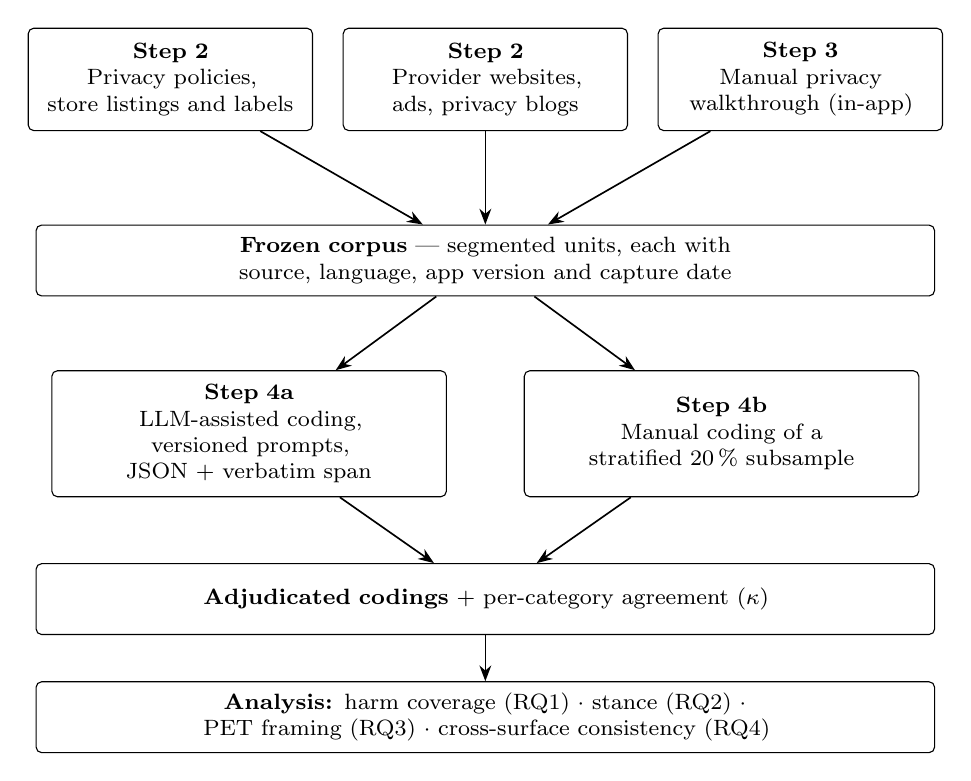
\begin{tikzpicture}[
  font=\footnotesize,
  src/.style ={draw, rounded corners=2pt, align=center, text width=34mm,
               minimum height=13mm, inner sep=3pt},
  proc/.style={draw, rounded corners=2pt, align=center, text width=48mm,
               minimum height=16mm, inner sep=3pt},
  wide/.style={draw, rounded corners=2pt, align=center, text width=112mm,
               minimum height=9mm, inner sep=3pt},
  arr/.style ={-{Stealth[length=2mm]}, semithick}
]
  \node[src] (s1) at (-4.0, 2.3)
    {\textbf{Step 2}\\Privacy policies,\\store listings and labels};
  \node[src] (s2) at ( 0.0, 2.3)
    {\textbf{Step 2}\\Provider websites,\\ads, privacy blogs};
  \node[src] (s3) at ( 4.0, 2.3)
    {\textbf{Step 3}\\Manual privacy\\walkthrough (in-app)};

  \node[wide] (corpus) at (0,0)
    {\textbf{Frozen corpus} --- segmented units, each with source, language,
     app version and capture date};

  \node[proc] (llm) at (-3.0,-2.2)
    {\textbf{Step 4a}\\LLM-assisted coding,\\versioned prompts,
     JSON $+$ verbatim span};
  \node[proc] (man) at ( 3.0,-2.2)
    {\textbf{Step 4b}\\Manual coding of a\\stratified 20\,\% subsample};

  \node[wide] (adj) at (0,-4.3)
    {\textbf{Adjudicated codings} $+$ per-category agreement ($\kappa$)};
  \node[wide] (ana) at (0,-5.8)
    {\textbf{Analysis:} harm coverage (RQ1) $\cdot$ stance (RQ2) $\cdot$
     PET framing (RQ3) $\cdot$ cross-surface consistency (RQ4)};

  \draw[arr] (s1) -- (corpus);
  \draw[arr] (s2) -- (corpus);
  \draw[arr] (s3) -- (corpus);
  \draw[arr] (corpus) -- (llm);
  \draw[arr] (corpus) -- (man);
  \draw[arr] (llm) -- (adj);
  \draw[arr] (man) -- (adj);
  \draw[arr] (adj) -- (ana);
\end{tikzpicture}
\caption{Overview of the study design. Step~1 (sampling) determines which apps
enter the three collection streams at the top.}
\label{fig:method}
\end{figure}

\subsection{Step 1: App Sampling}
\label{sec:sampling}

\paragraph{Platforms and market.}
Google Play and the Apple App Store, German storefront, German device locale.
Both platforms are covered because their structured disclosures differ (Data
Safety section versus Privacy Nutrition Labels) and RQ4 depends on that
difference.

\paragraph{Search.}
A fixed, pre-registered keyword list is used on both stores, in German and
English, because German listings routinely use English terms. The seed list
covers the two domains and their common synonyms: \emph{Fitness, Fitness
Tracker, Schrittz\"ahler, Aktivit\"atstracker, Schlaf-Tracker, Herzfrequenz,
Kalorienz\"ahler, Ern\"ahrungstagebuch, Workout} for the fitness domain, and
\emph{Periode, Zyklus, Zyklustracker, Menstruation, Eisprung, Fruchtbarkeit,
Kinderwunsch, period tracker, ovulation, fertility} for the fertility domain.
The list is frozen before collection; any addition is recorded in the change log
of the sampling protocol with its date and reason. Store categories considered
are \emph{Health \& Fitness} and \emph{Medical}.

\paragraph{Operationalising \enquote{highest rated}.}
\enquote{Highest rated} is ambiguous and is therefore fixed in advance. For each
keyword, the first 20 results in the store's default ordering are recorded
together with their average rating and rating count. The pooled, de-duplicated
candidate set is then filtered to apps with at least 1{,}000 ratings on the
platform in question --- below that, the average rating is noise --- and ranked
by average rating, with rating count as the tie-break. This makes the sample
\emph{highly rated among widely used apps} rather than \emph{rated highly by a
handful of people}, which is the intended reading.

\paragraph{Inclusion criteria.} An app is included if all of the following hold:
\begin{enumerate}[leftmargin=*,itemsep=1pt]
  \item it is available in the German storefront of at least one of the two
        platforms;
  \item it collects health, fitness, or body-related self-tracking data from the
        user or a paired device;
  \item it is free to install, so that the walkthrough can reach onboarding
        without a purchase;
  \item a privacy policy is reachable from the store listing;
  \item its interface is available in German or English.
\end{enumerate}

\paragraph{Exclusion criteria.} An app is excluded if any of the following hold:
\begin{enumerate}[leftmargin=*,itemsep=1pt]
  \item no privacy policy is reachable, or the link is dead at capture time
        (recorded as a finding, then excluded from text coding);
  \item it is a prescription DiGA or is marketed as a regulated medical device;
  \item it is a pure device companion with no tracking function of its own;
  \item account creation requires identity verification or payment, which the
        ethics rules in Section~\ref{sec:ethics} forbid;
  \item it duplicates an app already in the sample from the same provider under
        a different name.
\end{enumerate}

\paragraph{Sample size and stratification.}
The target is \textbf{50 apps} for document analysis, stratified as 30 fitness
and activity apps and 20 fertility and period apps. The fertility stratum is
deliberately over-represented relative to its market share: it is the domain
where the harm literature is most developed and where the consequences are most
concrete~\parencite{cao2024deleted,malki2024exploring,shipp2020period}, which
makes it the more informative half of a comparison. A \textbf{pilot of five
apps} (three fitness, two fertility) is run first to test the collection
protocol, the codebook, and the prompts; pilot apps are re-coded with the final
instruments and retained in the sample.

\paragraph{Freezing.}
Everything is recorded with a capture date and app version, and the corpus is
frozen on a stated date. Policies change; a moving corpus cannot be analysed.
The full record per app is specified in
\pathname{04_Study/App-Sample/sampling_protocol.md}.

\subsection{Step 2: Material Collection}

For every app in the sample, the following are collected, archived as both the
original file and extracted plain text, and given a stable document identifier:

\begin{enumerate}[leftmargin=*,itemsep=2pt]
  \item \textbf{Privacy policy}, in German if one is offered to a German user and
        in English otherwise; both if both exist, with the difference recorded.
  \item \textbf{Store listing}: full description text, plus the structured
        disclosure (Play Data Safety section, App Store Privacy Nutrition Label)
        captured as text and screenshot.
  \item \textbf{Provider website}: the service description, any dedicated privacy
        or security page, and any privacy-related blog or newsroom post.
  \item \textbf{Advertisements}, where encountered --- in-app ads shown during
        the walkthrough, and any ad creative reachable from the provider's own
        channels. Advertising is treated as a \emph{secondary} corpus: it is
        coded when found, but its absence for a given app is not itself a
        finding, because ad delivery cannot be systematically reproduced.
  \item \textbf{In-app privacy text}, from the walkthrough (Step~3).
\end{enumerate}

Each document is recorded with source type, language, URL, capture date,
SHA-256 hash of the archived file, and the app version it belongs to. Collection
is manual or uses officially permitted access; each store's terms are checked
before any automated retrieval, and manual capture is preferred where the terms
are restrictive.

\paragraph{Segmentation.}
Documents are split into coding units at heading and paragraph boundaries, with
list items as their own units. Units, not documents, are the unit of coding;
document-level counts are derived afterwards. This keeps a 40-page policy and a
three-line store blurb commensurable.

\subsection{Step 3: Privacy-Focused Cognitive Walkthrough}
\label{sec:walkthrough}

Walkthroughs are manual and are run on a \textbf{stratified subsample of 12
apps}, drawn from the top of the ranked sample so that the most-used apps are
covered. Unlike the document sample, the subsample is \emph{balanced}: six
fitness and six fertility apps, each domain split three on Android and three on
iOS. Balance is deliberate here, because RQ4 compares domains and platforms
against each other and an unequal subsample would confound that comparison with
sample size. Twelve is what a single analyst can walk through consistently
within the schedule while covering both platforms and both domains.

The method follows the cognitive walkthrough~\parencite{wharton1994cognitive},
with one adaptation: the tasks are \emph{privacy} tasks. For each task the
analyst walks the action sequence and asks Wharton et al.'s four questions ---
will the user try to achieve the right effect; will they notice that the correct
action is available; will they associate the correct action with the effect they
want; and, once the action is performed, will they see that progress is being
made. The tasks are:

\begin{enumerate}[leftmargin=*,itemsep=1pt]
  \item find out what data the app collects;
  \item find out what the app or provider \emph{derives} from that data;
  \item find out what happens if the data is exposed, and how incidents are
        handled;
  \item reach the privacy policy from inside the app;
  \item turn off sharing with third parties;
  \item export the data;
  \item delete the account and the data.
\end{enumerate}

Tasks 2 and 3 are the ones that matter for RQ1: they are expected to fail, and
the walkthrough records \emph{where} they fail. Each session follows the fixed
sequence in \pathname{04_Study/Instrument/walkthrough_protocol.md} --- store
listing captured before install, fresh install, no restored backup, screen
recording throughout, every consent and permission dialogue recorded verbatim,
taps-to-target counted from the home screen. Observation and interpretation are
written separately in the notes; only the observation is data.

Walkthroughs are run by a single analyst, which is a known weakness of
inspection methods~\parencite{nielsen1994heuristic}. It is mitigated by the
fixed protocol, the screen recordings (which make a second pass possible), and
by double-coding the walkthrough notes as part of the validation subsample.

\subsection{Step 4: Coding Framework}
\label{sec:framework}

Every coding unit is coded on three axes. The axes are independent: a unit can
carry codes on all three, or on none.

\paragraph{Axis A --- harm type and pathway (RQ1).}
The backbone is the Citron and Solove typology: physical, economic,
reputational, psychological, autonomy, discrimination, and relationship
harm~\parencite{citron2021harms}. Its seven categories were built for
adjudication, not for content analysis, so each is given an operational
definition, a positive example, and a counter-example in the codebook; a
category that cannot be given a counter-example is not codable and is merged or
dropped. On top of this, four \textbf{probe codes} capture the specific silences
identified in Section~\ref{sec:problem}: \textsc{inference},
\textsc{breach-consequence}, \textsc{incident-handling}, and
\textsc{concrete-consequence}. Finally, where a unit does describe a route to
harm, it is annotated with the stage of the Knabenhans et al.\ harm
pathway~\parencite{knabenhans2026harms} it refers to --- system component,
adversarial capability (distinguishing, tracking, inferring), or harm --- which
records whether providers describe mechanisms, capabilities, or outcomes.

\paragraph{Axis B --- stance (RQ2).}
For each harm code, one stance is assigned: \textsc{acknowledged} (the harm is
named as a real possibility), \textsc{hedged} (named but qualified into
improbability), \textsc{minimised} (named alongside a claim that defuses it
without substantiation), \textsc{deflected} (named but made the user's
responsibility), or \textsc{absent} (recorded at document level, not unit
level). \textsc{Absent} is a document-level and app-level judgement: it can only
be asserted after the whole corpus for that app has been coded.

\paragraph{Axis C --- PET framing (RQ3).}
Where a protective technology or practice is described, the unit is coded for
which of the three principles of Martin et al.\ it invokes --- limiting
third-party access, minimising raw data in favour of inferences, or on-device
processing~\parencite{martin2025cookies} --- and for whether the protection is
framed as \textbf{secrecy} (nobody else sees the data) or as \textbf{harm
prevention} (a specific bad outcome is prevented). A separate code marks
\textsc{reassurance-without-substance}: claims such as \enquote{your data is
safe with us} that carry no verifiable commitment.

The framework is deductive at the start and inductive at the edges: codes that
the corpus demands but the framework does not anticipate are added through
thematic analysis~\parencite{braun2006using}, each one triggering a new codebook
version with its rationale recorded.

\subsection{Step 4a: LLM-Assisted Coding}

The corpus is too large to code entirely by hand --- 50 apps across four or five
source types, with individual policies commonly running to several thousand
words~\parencite{mcdonald2008cost} --- and LLMs have been evaluated for exactly
this kind of policy analysis at scale~\parencite{rodriguez2024llm}. Existing tooling is not reused directly:
the OPP-115 scheme and Polisis classify \emph{data
practices}~\parencite{wilson2016creation,harkous2018polisis}, and have no harm
categories, so a purpose-built prompt pipeline over the codebook of
Section~\ref{sec:framework} is required. Their category sets are, however, used
as a cross-check that the corpus was segmented and parsed correctly.

The pipeline is constrained as follows:

\begin{itemize}[leftmargin=*,itemsep=2pt]
  \item \textbf{One prompt per axis}, not one prompt for everything. Each prompt
        file carries the header specified in
        \pathname{04_Study/Prompts/README.md}: task, version, date, exact model
        name and version, input, output schema, and what changed since the
        previous version.
  \item \textbf{Structured output.} The model returns JSON: unit identifier,
        codes assigned, and for each code a \emph{verbatim span} copied from the
        unit plus a confidence flag. A code without a span is discarded
        automatically.
  \item \textbf{Determinism and stability.} A single pinned model version,
        temperature 0, three independent runs per unit, majority vote across
        runs. The rate of disagreement between runs is itself reported as a
        measure of instrument stability.
  \item \textbf{No inference beyond the text.} The prompt instructs the model to
        code what is written, never what the provider presumably means --- the
        same rule that binds the human coder.
  \item \textbf{Logging.} Every run is entered in
        \pathname{04_Study/Prompts/run_log.md} with date, prompt version, model,
        document count, and anything that went wrong.
\end{itemize}

\subsection{Step 4b: Validation}
\label{sec:validation}

LLM output is treated as a measurement instrument that must be calibrated, not
as ground truth.

\begin{enumerate}[leftmargin=*,itemsep=3pt]
  \item \textbf{Agreement.} A stratified 20\,\% subsample of coding units ---
        drawn across both domains, both platforms, and all source types --- is
        coded manually by the author, blind to the model output. Agreement is
        computed per code with Cohen's $\kappa$~\parencite{cohen1960coefficient}
        and reported per category, not as a single pooled figure, because the
        rare categories are the interesting ones and a pooled figure hides them.
  \item \textbf{Threshold and remedy.} The target is $\kappa \geq 0.70$ per
        code. Where a code falls below it, the failure is diagnosed as either a
        codebook problem (ambiguous definition, missing counter-example) or a
        prompt problem; the relevant instrument is revised, its version
        incremented, and a fresh subsample drawn. Codes that cannot be brought
        above the threshold after two revisions are reported as unreliable and
        excluded from quantitative claims, with the reason stated.
  \item \textbf{Precision audit.} Independently of agreement, every code that
        enters the results is checked against its verbatim span; a span that
        does not support the code is discarded and counted. The resulting false
        positive rate is reported.
  \item \textbf{Second coder.} A second coder on a portion of the subsample
        would strengthen the design considerably; whether one can be arranged
        through the supervisor is one of the open points in
        Section~\ref{sec:openpoints}. If none is available, this is stated
        plainly as a limitation and reporting follows the norms for
        single-coder qualitative work in HCI, which require the reliability
        procedure to be described rather than a number to be
        claimed~\parencite{mcdonald2019reliability}.
\end{enumerate}

\subsection{Codebook and Coding Procedure}

The codebook lives in \pathname{04_Study/Codebook/} and is versioned. Every
category carries a definition, a positive example, and an explicit
counter-example; the counter-example is mandatory because without it neither a
human coder nor a model has a boundary, and both drift. The standing rules are:

\begin{enumerate}[leftmargin=*,itemsep=1pt]
  \item Code the text as written, never what the provider is assumed to mean.
  \item A unit may carry several codes; codes are not mutually exclusive across
        axes.
  \item Every code records source, verbatim quote, and location.
  \item When unsure, code it and flag it --- never silently drop it.
  \item Any change to a category produces a new codebook version with date,
        change, and reason in the version history.
\end{enumerate}

Disagreements between the manual and model codings are adjudicated by the author
against the verbatim span and the codebook; each adjudication is logged with the
rule that resolved it, and a pattern of adjudications against the same category
is treated as evidence that the category needs revision.

\subsection{Ethics and Data Handling}
\label{sec:ethics}

The study involves \textbf{no human subjects}. The material is public documents
and the researcher's own interaction with publicly available apps, so no ethics
approval is expected to be required. This will nevertheless be confirmed in
writing with the supervisor and the relevant RUB\,/\,MPI-SP contact before
collection starts, and the answer filed in \pathname{04_Study/Ethics/}. If the
scenario-based survey is later added as a second phase, it does require review,
and an application would have to be filed well in advance.

The practical rules for the walkthroughs are binding regardless of that answer:
throwaway accounts and synthetic data only; no real name, address, health data,
or payment details entered into any studied app; no account that requires
identity verification (such apps are excluded by
Section~\ref{sec:sampling}); each store's terms checked before any automated
collection. Screen recordings and archived documents are stored locally in
\pathname{05_Data/raw/}, which is excluded from version control; only derived,
non-identifying data is committed. Use of an LLM in the analysis is part of the
method and is declared as such, both in the methodology chapter and in the
statutory declaration on AI use.

\subsection{Limitations and Threats to Validity}

\paragraph{Absence is not intent.}
The study can establish that a harm type is not mentioned. It cannot establish
why. Silence may be a drafting convention, a legal risk decision, or a
deliberate omission, and the thesis will not attribute motive. This is a
boundary on the claims, not a flaw in the measurement.

\paragraph{A snapshot, not a trend.}
Policies, labels, and interfaces change continuously. The corpus is frozen on a
stated date and every claim is indexed to it. Longitudinal comparison is out of
scope.

\paragraph{Market and language.}
The German storefront determines the sample. Many providers operate
internationally and serve near-identical policies everywhere, but jurisdiction
shapes the text, and findings should not be read as global without
qualification. Where a policy exists in both German and English, the pair is
recorded, and any divergence between them is itself reportable.

\paragraph{Measurement error in the instrument.}
LLM coding is sensitive to prompt wording and is not perfectly reproducible even
at temperature 0. The mitigations are in Section~\ref{sec:validation}: pinned
model version, repeated runs with a reported disagreement rate, per-category
$\kappa$ against manual coding, mandatory verbatim spans, and a precision audit.
The agreement figures are reported whatever they turn out to be.

\paragraph{Single analyst.}
One person builds the sample, runs the walkthroughs, and does the manual coding.
Fixed protocols, screen recordings, versioned instruments, and a committed audit
trail are the compensating controls; a second coder, if one can be arranged,
would be better and is requested in Section~\ref{sec:openpoints}.

\paragraph{Coverage of the interface.}
Walkthroughs cover 12 of 50 apps and only the free tier. Privacy-relevant
content behind a paywall or a rarely used flow may be missed. The subsample is
drawn from the top of the ranking so that the apps most people actually use are
the ones inspected.

\paragraph{Advertising is opportunistic.}
Ad delivery is personalised and cannot be reproduced systematically, so the
advertising corpus is a secondary source. Presence of privacy claims in ads is
reportable; their absence is not.

\paragraph{The text is not the practice.}
Coding communication says nothing about whether the communication is true.
That question is answered by traffic and code analysis in existing
work~\parencite{arkalakis2024abandon,hudig2025intimate,huckvale2019assessment},
and the findings here should be read alongside it, not as a substitute for it.

\section{Timeline}

\begin{table}[htbp]
\centering
\begin{tabularx}{\textwidth}{@{}llX@{}}
\toprule
\textbf{Phase} & \textbf{Period} & \textbf{Deliverable} \\
\midrule
Literature review   & \todo{}  & Annotated reading list \\
Proposal            & \todo{}  & This document, approved \\
Sampling            & \todo{}  & App sample, documented \\
Material collection & \todo{}  & Corpus of privacy texts \\
Walkthroughs        & \todo{}  & Walkthrough notes \\
Analysis            & \todo{}  & Coded dataset, results \\
Writing             & \todo{}  & Thesis draft \\
Submission          & \todo{}  & Final thesis \\
\bottomrule
\end{tabularx}
\caption{Planned schedule.}
\label{tab:timeline}
\end{table}

\section{Expected Contributions}
\label{sec:contributions}

At the end of this work the following will exist, none of which exists now.

\begin{enumerate}[leftmargin=*,itemsep=5pt]
  \item \textbf{The first systematic map of harm communication in health
    tracking apps.} A coded account, across 50 fitness and fertility tracking
    apps in the German market, of which privacy harm types providers name, which
    they minimise, and which never appear --- broken down by harm category, by
    domain, and by communication surface. This answers the question the harm
    literature and the tracker-measurement literature both leave open.

  \item \textbf{A quantified account of four specific silences.} Per-app and
    per-surface figures for whether inference, breach consequences, incident
    handling, and any concrete consequence for the user are mentioned at all.
    This is the empirical core: it converts the observation motivating the
    thesis into a number that can be cited, contested, and re-measured later.

  \item \textbf{A reusable harm-communication codebook.} A versioned coding
    instrument that operationalises the Citron and Solove
    typology~\parencite{citron2021harms} for corporate privacy text --- each
    category with a definition, a positive example, and a counter-example ---
    extended with the Knabenhans et al.\ pathway
    annotation~\parencite{knabenhans2026harms} and a PET-framing axis derived
    from Martin et al.~\parencite{martin2025cookies}. Existing annotation
    schemes for privacy policies code data practices; this one codes harm, and
    is designed to be applied to other domains unchanged.

  \item \textbf{A privacy-focused cognitive walkthrough instrument.} An
    adaptation of Wharton et al.'s
    procedure~\parencite{wharton1994cognitive} in which the user goals are
    privacy goals --- find out what is inferred, find out what happens after a
    breach, stop third-party sharing, delete everything --- with a fixed task
    sequence and record sheet. It is reusable by anyone inspecting privacy
    communication in an interface rather than in a document.

  \item \textbf{A reproducible LLM-assisted analysis pipeline, honestly
    reported.} Versioned prompts, a pinned model, structured output with
    mandatory verbatim spans, a run log, and a validation report giving Cohen's
    $\kappa$ per category against manual coding together with the run-to-run
    disagreement rate and the precision audit. Whatever the agreement figures
    turn out to be, they are published with the results --- which is what makes
    the pipeline usable by the next person rather than only by its author.

  \item \textbf{Design and policy implications.} Concrete statements about where
    harm-relevant information is missing from the surface on which users
    actually decide, and what a disclosure regime built around data practices
    does not cause providers to say. If a second phase is pursued, the coded
    corpus supplies realistic, evidence-based stimulus material for the
    scenario-based survey described in the original thesis offer.
\end{enumerate}

\section{Open Points for Confirmation}
\label{sec:openpoints}

The methodology above commits to a decision on every question that was still
open after the meeting of 4~September~2026 and the written input of
5~September~2026, so that work can proceed without waiting. Each decision and
its rationale is listed here for the supervisor to confirm or overturn. Where a
decision is overturned, the affected part of Section~\ref{sec:method} is the
only thing that changes.

\begin{enumerate}[leftmargin=*,itemsep=5pt]
  \item \textbf{Scope: document and interface analysis, not a user survey.}
    The written input of 5~September lists only document and interface sources,
    which settles the question raised in the meeting notes. The scenario-based
    online survey from the original thesis offer is treated as a possible second
    phase and is out of scope here (Section~\ref{sec:problem}).
    \emph{Confirm that this closes the question.}

  \item \textbf{Harm taxonomy: Citron and Solove as the backbone, Knabenhans et
    al.\ as the pathway annotation.} The seven categories give comparable,
    citable buckets; the harm-tree stages record whether a provider is
    describing a mechanism, a capability, or an outcome. The two are used
    together rather than merged, so that neither loses its original meaning.
    \emph{Confirm this is the intended reading of the two papers.}

  \item \textbf{\enquote{Highest rated} operationalised as: at least 1{,}000
    ratings, then ranked by average rating.} Without a minimum rating count,
    \enquote{highest rated} selects obscure apps with a handful of five-star
    reviews. \emph{Confirm the threshold, or name a different one.}

  \item \textbf{Sample size: 50 apps, stratified 30 fitness\,/\,20 fertility, as
    the final target rather than a pilot.} A separate five-app pilot is run
    first to test the instruments. \emph{Confirm 50 is the target and not a
    first pass towards something larger.}

  \item \textbf{Walkthroughs on 12 of the 50 apps, balanced six fitness\,/\,six
    fertility and three Android\,/\,three iOS per domain.} Twelve is what one
    analyst can do consistently inside the schedule; the balance keeps the
    domain and platform comparisons in RQ4 from being confounded with sample
    size. \emph{Confirm the subsample size and the balanced split, or state that
    every sampled app must be walked through --- which would require reducing
    the document sample.}

  \item \textbf{Advertisements and privacy blogs as a secondary corpus.} Both
    are coded where found, but absence is not treated as a finding, because ad
    delivery cannot be reproduced systematically.
    \emph{Confirm that they need not be in the core corpus.}

  \item \textbf{Language: German storefront, German policy where offered,
    English otherwise, with divergences recorded.}
    \emph{Confirm this is acceptable, and whether quoted material should be
    translated in the thesis or left in the original with a translation in a
    footnote.}

  \item \textbf{A second coder.} The validation design would be materially
    stronger with a second coder on part of the subsample. \emph{Can one be
    arranged through the chair or MPI-SP?} If not, the limitation is reported as
    such (Section~\ref{sec:validation}).

  \item \textbf{Choice of model for the LLM-assisted coding.} The pipeline
    requires a pinned model version that will remain available for the duration
    of the thesis and that may be used on this material. \emph{Confirm whether a
    particular model or an institutional API should be used, or whether the
    choice is the author's.}

  \item \textbf{Ethics.} No human subjects are involved, so no review is
    expected to be needed. \emph{A written confirmation from the supervisor and
    the relevant RUB\,/\,MPI-SP contact is requested before collection starts},
    to be filed in \pathname{04_Study/Ethics/}.
\end{enumerate}


%---------------------------- References ------------------------------
\newpage
\printbibliography[heading=bibintoc,title={References}]

\end{document}
